\chapter{Аналитическая часть}

\section{Постановка задачи}

В соотвествии с техническим заданием на курсовую работу необходимо разработать загрузаемый модуль ядра  для получения информации о приоритетах, времени выполнения и простоя, выделенной виртуальной памяти, сегментах разделяемой памяти, программных каналов, семафорах и сигналов процессов. Для поставленной задачи необходимо:

\begin{itemize}
	\item провести анализ структур и функций ядра, предоставляющих возможность реализовать поставленную задачу;
	\item провести анализ подходов к перехвату функций; 
	\item провести анализ методы передачи информации из простраства ядра в простраство пользователя и наоборот;
	\item разработать алгоритмы и структуру загружаемого модуля ядра, в соотвесвии с поставленной задачей;
	\item спроектировать и реализовать загрузаемый модуль ядра;
	\item исследовать работу реализованного модуля ядра.
\end{itemize}

К разрабатываемой программе предъявляются следующие требования:

\begin{itemize}
	\item взаимодействие с загружаемым модулем должно происходить из пространства пользователя; 
	\item необходимо передавать данные из пространства ядра в пространство пользователя или наоборот.
\end{itemize}

\clearpage

\section{Анализ структур и функций ядра}

\subsection{Структура процесса}

Каждый процессе в ядре описывается структурой \texttt{struct task\_struct}, которая содержит информацию, необходимую для управления процессом и называется дескриптором процесса, описана в файле \texttt{<linux/sched.h>}.

Множество процессов в Linux-системе представляет собой совокупность структур \texttt{struct task\_struct}, которые взаимосвязаны по средством  кольцевого двусвязанного списока. 
Максимальное количество процессов, которое может быть создано, ограничивается только объемом физической памяти.
В листинге~\ref{lst:structs:task-1} представлены необходимые для решения задачи фрагменты структуры \texttt{task\_struct}~\cite{structs:task}.

\lstinputlisting[label=lst:structs:task-1,caption=Структура struct task\_struct, firstline=0,lastline=18]{./structs/task_struct.c}

\lstinputlisting[label=lst:structs:task-2,caption=Структура struct task\_struct, firstline=19,lastline=52]{./structs/task_struct.c}

\lstinputlisting[label=lst:structs:task-3,caption=Структура struct task\_struct, firstline=53]{./structs/task_struct.c}

Подробное описание представленного фрагмента структуры \texttt{task\_struct}.

Cостояние процесса опредяеляется следующими члены, значение которых представлены в листинге~\ref{lst:structs:states-1}:
\begin{enumerate}
	\item \texttt{\_\_state} --- состояние процесса;
	\item \texttt{exit\_state} --- состояние завершение процесса.
\end{enumerate}

\lstinputlisting[label=lst:structs:states-1,caption=Макросы состояния процесса, firstline=0,lastline=13]{./structs/states.c}
\lstinputlisting[label=lst:structs:states-2,caption=Макросы состояния процесса, firstline=14]{./structs/states.c}

\clearpage

Идентификатор процесса и члены, представляющий родство процесса:
\begin{enumerate}
	\item \texttt{pid} --- уникальный идентификатор процесса;
	\item \texttt{ppid} --- идентификатор процесса-родителя;
	\item \texttt{tgid} --- идентификатор лидера группы потоков;
	\item \texttt{real\_parent} --- указывает на родительский процесс, если родительский процесс завершился, то указывает на процесс, pid которого равен 1;
	\item \texttt{parent} --- родительский процесс;
	\item \texttt{children} --- двусвязанный список дочерних процессов; 
	\item \texttt{sibling} --- двусвязанный список, используещиеся для связанности дочерних процессов с родительским процессом, которая представлена на рисунке~\ref{img:structs:children-linkage}; 
	\item \texttt{group\_leader} --- процесс--лидер группы процессов. 
\end{enumerate}

\begin{figure}[h]
	\centering
	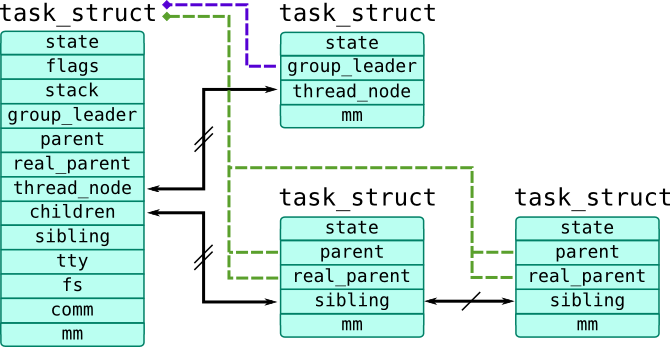
\includegraphics[height=0.3\textheight]{img/children-linkage.png}
	\caption{Связанность дочерных процессов с родительским процессом}
	\label{img:structs:children-linkage}
\end{figure}

\clearpage

Приоритет и алгоритм планировщика задач, описываются в следующих членах:
\begin{enumerate}
	\item \texttt{prio} --- приоритет процесса, которое используется планировщиком задач при выборе процесса. Чем ниже значение данной переменной, тем выше приоритет процесса. Диапазон значений от 0 до 139, то есть MAX\_PRIO. Данный диапазон делится на два интервала: 
	\begin{itemize}
		\item 0 -- 99 --- приоритет процессов в реальном времени;
		\item 100 -- 139 --- приоритет обычных процессов, по умолчанию 120;
	\end{itemize}
	Особое внимание необходимо уделить процессу с приоритетом 0 --- migration, который перераспределяет процессы между ядрами процессора. У таких процессов алгоритм планирования устанавливается FIFO, по причине того, что данный процесс имеет наивысший приоритет и ему необходимо выполнится от начало и до конца;
	\item \texttt{static\_prio} --- приоритет процесса, который не изменяется при работе планировщика задач, однако оно может быть изменено с использованием системного вызова nice;
	\item \texttt{normal\_prio} --- приоритет процесса, который зависит от статического приоритета и алгоритма планировщика задач; 
	\item \texttt{rt\_proirity} ---  приоритет процессов в реальном времени;
	\item \texttt{policy} --- алгоритма планирования, значение которого представлены в листинге~\ref{lst:structs:policy}.
\end{enumerate}

\lstinputlisting[label=lst:structs:policy,caption=Макросы значений policy]{./structs/policy.c}

\clearpage

Время выполнения описывается следующими членами:
\begin{enumerate}
	\item \texttt{utime} --- время процесса, проведенное в режиме пользователя;
	\item \texttt{stime} --- время процесса, затраченное на выполнение системных вызовов;
	\item \texttt{start\_time} --- время создания процесса;
	\item \texttt{start\_boottime} --- время ожидания процесса.
\end{enumerate}

\subsection*{struct sched\_info}

\texttt{struct sched\_info} ---  структрура, которая предоставляет информацию о планировании процесса, представлена в листиге~\ref{lst:structs:sched_info}.

\lstinputlisting[label=lst:structs:sched_info,caption=struct sched\_info]{./structs/sched_info.c}

Подробное описание представленной структуры sched\_info:
\begin{enumerate}
	\item \texttt{pcount} --- количетство запусков процесса на исполнение центральным процессом;
	\item \texttt{run\_delau} --- количество времени, проведенного в ожидании на исполнение;
	\item \texttt{last\_arrive} --- время последнего запуска процесса на исполнение центральным процессором;
	\item \texttt{last\_queued} --- время последнего процесса в очередь на исполнение  центральным процессором.
\end{enumerate}

\subsection{Адресное пространство процесса}

\texttt{struct~mm\_struct} --- структура, которая описывает адресное пространство процесса и описана в файл \texttt{<linux/mm\_types.h>}.
У \texttt{task\_struct} есть два указателя \texttt{mm} и  \texttt{active\_mm} на струкртуру \texttt{mm\_struct}, использущиеся во время выполнения процесса. Для обычных процессов значения этих двух переменных-указателей одинаковы. Однако потоки не владеют адресным пространством, поэтому \texttt{mm} имеет значение NULL, a \texttt{active\_mm} указывает на дескриптор адресного пространства процесса, создавшего поток.
Фрагмент этой структуры представлен в листинге~\ref{lst:structs:mm_struct-1}.

\lstinputlisting[label=lst:structs:mm_struct-1,caption=struct mm\_struct, firstline=0,lastline=21]{./structs/mm_struct.c}
\lstinputlisting[label=lst:structs:mm_struct-2,caption=struct mm\_struct, firstline=22]{./structs/mm_struct.c}

\texttt{struct vm\_area\_struct} --- структура, которая описывает непрерывную область адресного пространства процесса.
У объекта {mm\_struct} содержит указать на струтктуру  \texttt{vm\_area\_struct}. Фрагмент этой структуры предствален в листинге~\ref{lst:structs:vm_area_struct-1}.

\lstinputlisting[label=lst:structs:vm_area_struct-1,caption=struct vm\_area\_struct,firstline=0,lastline=7]{./structs/vm_area_struct.c}
\lstinputlisting[label=lst:structs:vm_area_struct-2,caption=struct vm\_area\_struct,firstline=8]{./structs/vm_area_struct.c}

\subsection{Сигналы}
Сигнал --- способ информирвоания процесса ядром о происшествии какого-то события. 
Сигнал означает, что произошло событие, но ядро не сообщает сколько таких событий произошло. 
Если возникате несколько однотипных событий, процессу будет подан только один сигнал.

\texttt{struct~signal\_struct} --- структура, которая описывает сигнал процесса. Объект \texttt{task\_struct} содержит указатель на данную структуру. Данная структура представлена в листинге~\ref{lst:structs:signal_struct}.

\clearpage

\lstinputlisting[label=lst:structs:signal_struct,caption=struct sighand\_struct, firstline=27, lastline=48]{./structs/signals.c}

\texttt{struct sighand\_struct} --- структура, которая описывает обработчики сигналов процесса. 
Эта структура описана в файле \texttt{<linux/sched/signal.h>}.
У объекта \texttt{task\_struct}содержит указатель на данную струтктуру.
Эта структура представлена в листинге~\ref{lst:structs:sighand_struct}.

\texttt{struct k\_sigaction } --- структура, которая описывает обработчик сигнала процесса.
Эта структура представлена в листинге~\ref{lst:structs:sigaction}.

\clearpage

\lstinputlisting[label=lst:structs:sighand_struct,caption=struct sighand\_struct, firstline=0, lastline=6]{./structs/signals.c}

\lstinputlisting[label=lst:structs:sigaction,caption=struct k\_sigaction и struct sigaction, firstline=8, lastline=20]{./structs/signals.c}

Для работы с сигналами процессу предоставляется следующие системные вызовы.

Системный вызов \texttt{signal()} устанавливает обработчик на указанный сигнал. Важно отметит, что процесс имеет 64 сигналов и у каждого из них есть обработчики по умолчанию. В листинге~\ref{lst:structs:signal} пресдтавлен данный системный вызов.

\lstinputlisting[label=lst:structs:signal,caption=Системный вызов signal(), firstline=86, lastline=86]{./structs/signals.c}

\clearpage

В качестве параметров передаются:
\begin{itemize}
	\item \texttt{sig} --- номер сигнала;
	\item \texttt{handler} --- адрес функции, которая должна быть выполнена при поступлении указанного сигнала.
\end{itemize}

Системный вызов возвращает указатель на предыдущий обработчика данного сигнала, который можно использовать для восстановления обработчика. 
Вместо адреса обработчика можно указать 0 или 1. 
Если был указан 0, то при поступлении сигнала выполнение будет прервано. 
Если была указана 1, то сигнал будет проигнорирован. 

Системный вызов \texttt{kill()} отправляет сигнал указанному процессу. В листинге~\ref{lst:structs:kill} представлен данный системный вызов.

\lstinputlisting[label=lst:structs:kill,caption=Системный вызов kill(), firstline=87, lastline=87]{./structs/signals.c}

В качестве парамероа передаются:
\begin{itemize}
	\item pid --- уникальный идентификатор процесса, которому будет отправлен сигнал;
	\item sig --- номер сигнала.
\end{itemize}

Если вместо pid указать 0, то сигнал будет послал  всем процессам. 
Если вместо pid указать -1, то ядро  передает сигнал всем процессам, идентификатор пользователя которых равен идентификатору текущего  процесса, который посылает сигнал.

\subsection{Семафоры}

Linux поддерживает наборы считающих семафаров, которые семантически представлены в системе массивами и доступ к отдельному семафору осуществляется по номеру, начиная с 0. 
Основным свойством набора семафоров является возможность одной неделимой операцией изменить значения всех или части семафоров набора

Для описания всех семафоров в ядре имеется таблица семафоров, в которой отслеживаются все созданные наборы семафоров, структруа \texttt{struct semid\_ds}. Данная структура предаставлена в листинге~\ref{lst:structs:semid_ds}.

\lstinputlisting[label=lst:structs:semid_ds,caption=struct semid\_ds, firstline=0,lastline=10]{./structs/semafores.c}

Если несколько семафоров объединены в массив, то этот массив является набором семафором. 
\texttt{structs sem\_array} --- структура, которая описывает набор семафоров. Данная структура представлена в листинге~\ref{lst:structs:sem_array}.

\lstinputlisting[label=lst:structs:sem_array,caption=struct sem\_array, firstline=27,lastline=38]{./structs/semafores.c}

В двух структурах есть схожие поля, которые имеют одно и тоже назначение. Данные поля описаны ниже:
\begin{enumerate}
	\item \texttt{sem\_perm} --- информация о доступе к множеству семафоров, включая права доступа, и создателе семафора;
	\item \texttt{sem\_otime} --- время последней операции \texttt{semop()};
	\item \texttt{sem\_ctime} --- время последнего изменения структуры;
	\item \texttt{sem\_base} --- указатель на первый семафор в массиве;
	\item \texttt{sem\_nsems} --- количество семафоров в массиве.
\end{enumerate}


В \texttt{struct semid\_ds} и \texttt{struct sem\_array} есть указатель на структуру \texttt{struct sem}, которая описывает семафор. Данная структура представлена в листинге~\ref{lst:structs:sem}.

\lstinputlisting[label=lst:structs:sem,caption=struct sem, firstline=18,lastline=25]{./structs/semafores.c}

Подробнее описание полей струтктуры:
\begin{enumerate}
	\item \texttt{sempid} --- идентификатор процесса, проделавшего последнюю операцию;
	\item \texttt{semval} --- текущее значние семафора;
	\item \texttt{sem\_otime} --- время последней операции \texttt{semop()}.
\end{enumerate}

В Linux имеются системные вызовы для создания, изменение управляющих паарметров и уничтожения набора семафора, выполнения операций на семафорах. Данные системные вызовы поиманы ниже.

Системный вызов \texttt{semget()} создает новый набор семафоров или открывает уже существующий набор семафоров. Данный системный вызов представлен в листинге~\ref{lst:structs:semget}.

\lstinputlisting[label=lst:structs:semget,caption=Системный вызов semget(), firstline=89,lastline=89]{./structs/semafores.c}

В качестве параметров принимает:
\begin{itemize}
	\item \texttt{key} --- целочисленное значение, позволяющее несвязанным процессам обращаться к одному и тому же семафору;
	\item \texttt{nsems} --- количество семафоров, масимально значение которого равно значению макроса \texttt{SEMMSL};
	\item \texttt{semflg} --- результат побитого сложения прав доступа к семафору и \texttt{IPC\_CREATE}.
\end{itemize}

В случае успешного завершения системный вызов возвращает идентификатор семафора, а в случае неудачи возвращается -1. 
Существует особое значение ключа семафора --- \texttt{IPC\_PRIVATE}, которое предназначено для создания семафора, доступ к которому получает только сам процесс и процессы, порожденные процессом, создавшим семафор.

Допустимые флаги:
\begin{itemize}
	\item \texttt{IPC\_CREAT} создает набор семафоров, если его еще не было в системе;
	\item \texttt{IPC\_EXCL} при использовании вместе с \texttt{IPC\_CREAT} вызывает ошибку, если семафор уже
	существует. Сам по себе \texttt{IPC\_EXCL} бесполезен, но вместе с \texttt{IPC\_CREAT} он дает средство
	гарантировать, что ни одно из существующих множеств семафоров не открыто для доступа.
\end{itemize}

Системный вызов \texttt{semctl()} используется для осуществления управления множеством семафоров. 
Данный системный вызов представлен в листинге~\ref{lst:structs:semctl}.

\lstinputlisting[label=lst:structs:semctl,caption=Системный вызов semctl(), firstline=90,lastline=90]{./structs/semafores.c}

В качетве параметров передаются:
\begin{itemize}
	\item \texttt{semid} ---  идентификатор набора семафоров;
	\item \texttt{semnum} --- номер семафора в наборе семафоров;
	\item \texttt{cmd} --- команда, которая будет выполнена над набором семафоров;
	\item \texttt{arg} --- объединение \texttt{semun}.
\end{itemize}

Доступные команды над набором семафоров:
\begin{enumerate}
	\item \texttt{IPC\_STAT} --- возвращается стурктура \texttt{semid\_ds} для множества и запоминает ее по адресу аргумента  \texttt{buf} в объединении \texttt{semun};
	\item \texttt{IPC\_SET} --- устанавливает значение элемента \texttt{ipc\_perm} структуры \texttt{semid\_ds} для множества;
	\item \texttt{IPC\_RMID} --- удаляет множество из ядра;
	\item \texttt{GET\_ALL} --- возвращает значение всех семафоров множества, целые значения запоминаются в массиве элементов \texttt{unsigned short}, на который указывает член объединения \texttt{array};
	\item \texttt{GETNCNT} --- выдает число процессов, ожидающих ресурсов в данный момент;
	\item \texttt{GETPID} --- возвращает PID процесса, выполнившего последний вызов \texttt{semop()};
	\item \texttt{GETVAL} --- возвращает значение одного семафора из множества;
	\item \texttt{GETZCNT} --- возвращает число процессов, ожидающих 100\% освобождения ресурса;
	\item \texttt{SETALLM} --- устанавливает значения семафоров множества, взятые из элемента \texttt{array} объединения \texttt{args};
	\item \texttt{SETVAL} --- устанавливает значение конкретного семафора множества как элемент \texttt{val} объединения \texttt{args}.
\end{enumerate}

Объединение \texttt{union semun} представлено в листинге~\ref{lst:structs:semun}.

\lstinputlisting[label=lst:structs:semun,caption=union semun, firstline=93,lastline=97]{./structs/semafores.c}

Системный вызов \texttt{semop()} выполняет операцию на наборе семафоров. Данный системный вызов представлен в листинге~\ref{lst:structs:semop}.

\lstinputlisting[label=lst:structs:semop,caption=Системный вызов semop(), firstline=91,lastline=91]{./structs/semafores.c}

В качетве параметров передаются:
\begin{itemize}
	\item \texttt{semid} --- идентификатор набора семафоров;
	\item \texttt{sop} --- указатель на структуру операции на семафоре;
	\item \texttt{nsop} --- количетсво операций в этом массиве.
\end{itemize}

Структура \texttt{struct sembuf}, которая предназначена для описания выполнения операции на семафоре.
Данная структура представлена в листинге~\ref{lst:structs:sembuf}.

\lstinputlisting[label=lst:structs:sembuf,caption=struct sembuf, firstline=12,lastline=16]{./structs/semafores.c}

Подробное описание данной структуры:
\begin{enumerate}
	\item \texttt{sem\_num} ---  номер семафора в наборе семафоров;
	\item \texttt{sem\_op} --- выполняемая операция (положительное, отрицательное число или нуль);
	\item \texttt{sem\_flg} --- флаги.
\end{enumerate}

Если \texttt{sem\_op} отрицателен, то его значение вычитается из семафора. Это соответствует получению ресурсов, которые контролирует семафор. Если \texttt{IPC\_NOWAIT} не установлен, то вызывающий процесс блокируется, пока семафор не выдаст требуемое количество ресурсов. Если \texttt{sem\_op} положителен, то его значение добавляется к семафору. Это соответствует возвращению ресурсов множеству семафоров приложения. Если \texttt{sem\_op} равен 0, то вызывающий процесс будет блокирован, пока значение семафора не станет 0. Это соответствует ожиданию того, что ресурсы будут использованы на 100\%.

\subsection{Сегмента разделямой памяти}

Разделяемая память является средством передачи информации от процесса к
процессу. 
Разделяемая память (сегменты разделяемой памяти) была разработана для сокращения времени передачи сообщений за счет исключения необходимости копировать текст сообщения из пространства пользователя в пространство ядра. Это обеспечивается за счет возможности подключения разделяемого сегмента к адресному пространству процесса, а именно за счет возможности получения процессом указателя на разделяемый сегмент.
Аналогично программным каналам разделяемые сегменты создаются в разделяемой памяти, которой является область данных ядра системы. В отличие от программных каналов разделяемая память не имеет встроенных средств взаимоисключения и, как правило, используется совместно с семафорами.
Аналогично семафорам дескрипторы всех разделяемых сегментов находятся в системной таблице разделяемой памяти ядра системы.

Структура \texttt{struct shmid\_ds}, которая описывает системную таблицу разделяемой памяти. Данная структура представлена в листинге~\ref{lst:structs:shmid_ds}.

\lstinputlisting[label=lst:structs:shmid_ds,caption=struct shmid\_ds, firstline=0,lastline=10]{./structs/shm.c}

Подробное описание полей структуры:
\begin{enumerate}
	\item \texttt{shm\_perm} ---  информация о доступе к разделямой памяти, вклбчая права доступа и создетеля сегмента раздаелямой памяти;
	\item \texttt{shm\_segsz} --- раздел сегмента в байтах;
	\item \texttt{shm\_atime} --- время последнего поключения;
	\item \texttt{shm\_dtime} --- время последнего отключения;
	\item \texttt{shm\_ctime} --- время последнего изменения;
	\item \texttt{shm\_cpid} --- идентификатор процесса--создателя;
	\item \texttt{shm\_lpid} --- идентификатор последнего пользователя;
	\item \texttt{shm\_nattch} --- число процессов, привязанных к сегменту разделяемой памяти.
\end{enumerate}

В Linux имеются системные вызовы ля создания разделяемой памяти, изменения управляющих параметров созданного сегмента, подключения сегмента к адресному пространству процесса, т.е. получения указателя на него и отключения сегмента разделяемой памяти от адресного пространства процесса. 

Системный вызов \texttt{shmget()} создает новый разделяемый сегмент или, если сегмент уже существует, то права доступа подтверждаются.
Системный вызов возвращает в случае успеха идентифкатор сегмента разделяемой памяти, иначе -1. 
Данный системный вызов представлен в листинге~\ref{lst:structs:shmget}. 

\lstinputlisting[label=lst:structs:shmget,caption=Системный вызов shmget(), firstline=12,lastline=12]{./structs/shm.c}

В качестве параметров принимаются:
\begin{itemize}
	\item \texttt{key} --- целочисленное значение, позволяющее несвязанным процессам обращаться к одному и тому же сегменту разделяемой памяти;
	\item \texttt{size} --- размер памяти в байтах, которое будет выделено;
	\item \texttt{flag} --- результат побитого сложения прав доступа к сегменту разделяемой памяти и \texttt{IPC\_CREATE}.
\end{itemize}

Доступные флаги при создании сегмента разделяемой памяти:
\begin{enumerate}
	\item \texttt{IPC\_CREAT} служит для создания нового сегмента. Если этого флага нет, то функция \texttt{shmget()} будет искать сегмент, соответствующий ключу key и затем проверит, имеет ли пользователь права на доступ к сегменту.;
	\item \texttt{IPC\_EXCL} используется совместно с \texttt{IPC\_CREAT} для того, чтобы не создавать существующий сегмент заново.
\end{enumerate}

Системный вызов \texttt{shmctl()} изменяет управляющие параметры сегмента разделямой памяти. Системный вызов возвращает указатель на сегмент разделяемой памяти, иначе возвращается -1.
Данный системный вызов представлен в листинге~\ref{lst:structs:shmсtl}.

\lstinputlisting[label=lst:structs:shmсtl,caption=Системный вызов shmсtl(), firstline=13,lastline=13]{./structs/shm.c}

В качестве параметров принимаются:
\begin{itemize}
	\item \texttt{shmid} --- идентификатор сегмента разделяемой памяти;
	\item \texttt{cmd} --- команда, которая будет выполнена над сегментом разделяемой памяти;
	\item \texttt{buf} --- указатель на дескриптор в таблице сегментов разделяемой памяти.
\end{itemize}

Доступные команды над сегментом разделяемой памяти:
\begin{enumerate}
	\item \texttt{IPC\_STAT} --- идентификатор сегмента разделяемой памяти;
	\item \texttt{IPC\_SET} --- устанавливает значение \texttt{ipc\_perm}--элемента структуры \texttt{shmid\_ds}. Сами
	величины берет из аргумента \texttt{buf};
	\item \texttt{IPC\_RMID} --- помечает сегмент для удаления.
\end{enumerate}

Команда \texttt{IPC\_RMID} в действительности не удаляет сегмент из ядра, а только
помечает для удаления. Настоящее же удаление не происходит, пока последний процесс, привязанный к сегменту, не отвяжется от него как следует. Конечно, если ни один процесс не привязан к сегменту на данный момент, удаление осуществляется немедленно.

Системный вызов \texttt{shmat()} привязывает процесс к сегменту разделяемой памяти. В случае успеха возвращает адрес сегмента разделяемой памяти, иначе возвращается -1.
Данный системный вызов рпедставлен в листинге~\ref{lst:structs:shmat}.

\lstinputlisting[label=lst:structs:shmat,caption=Системный вызов shmat(), firstline=14,lastline=14]{./structs/shm.c}

В качестве параметров принимаются:
\begin{itemize}
	\item \texttt{shmid} --- идентификатор сегмента разделяемой памяти;
	\item \texttt{shmaddr} --- адресс сегмента разделяемой памяти, которому необходимо привязаться, если NULL, то ядро пытается найти
	нераспределенную область. Если значение shmaddr не равно NULL, а в \texttt{shmflg} указан флаг \texttt{SHM\_RND}, то
	подключение производится по адресу \texttt{shmaddr}, округлённому до ближайшего значения кратного \texttt{SHMLBA}.
	В противном случае \texttt{shmaddr} должно быть выровнено по адресу страницы, к которому производится подключение;
	\item \texttt{shmflg} --- флаги прав доступа к сегменту.
\end{itemize}

Системный вызов \texttt{shmdt()} отвязывает процесс от сегмента разделяемой памяти по указанному адресу. Системный вызов в случае успеха возвращает 0, иначе -1. Данный системный вызов представлен в листинге~\ref{lst:structs:shmdt}.

\lstinputlisting[label=lst:structs:shmdt,caption=Системный вызов shmdt(), firstline=15,lastline=15]{./structs/shm.c}

После того, как разделяемый сегмент памяти больше не нужен процессу, ондолжен быть отсоединен вызовом \texttt{shmdt()}. Как уже отмечалось, это не то же самое, что удаление сегмента из ядра. После успешного отсоединения значение
элемента \texttt{shm\_nattch} структуры \texttt{shmid\_ds} уменьшается на 1. Когда оно достигает 0, ядро физически удаляет сегмент.

\subsection{Программные каналы}

Канал представляет собой средство связи стандартного вывода одного процесса со стандартным вводом другого. 
Когда процесс создает канал, ядро устанавливает два файловых дескриптора для пользования этим каналом. Один такой дескриптор используется, чтобы открыть путь ввода в канал (запись), в то время как другой применяется для получения данных из канала (чтение). В этом смысле, канал мало применим практически, так как создающий его процесс может использовать канал только для взаимодействия с самим собой.

Программные каналы бывают именованные и неименованные. 
Неименованные программные каналы могут использоваться для обмена сообщениями между процессами родственниками. В отличие от именованных программных каналов неименованные не имеют идентификатора, но имеют дескриптор. Процесс--потомок наследует все дескрипторы открытых файлов процесса--предка, в том числе и неименованных программных каналов. Программные каналы имеют встроенные средства взаимоисключения --- массив файловых дескрипторов: из канала нельзя читать, если в него пишут, и в канал нельзя писать, если из него читают.

Системный вызов \texttt{pipe()} создает неименованный программный канал. В качетве параметра принимает массив из двух целых, которые связаны между собой. Данный системный вызов представлен в листинге~\ref{lst:structs:pipe}.

\lstinputlisting[label=lst:structs:pipe,caption=Системный вызов pipe(), firstline=1,lastline=1]{./structs/pipe.c}

Системный вызов \texttt{pipe2()} создает неименованный программный канал, также как и \texttt{pipe()}. В качетве параметра принимает в отличик от \texttt{pipe()} флаги прав доступа. Данный системный вызов представлен в листинге~\ref{lst:structs:pipe2}.

\lstinputlisting[label=lst:structs:pipe2,caption=Системный вызов pipe2(), firstline=2,lastline=2]{./structs/pipe.c}

Системный вызов \texttt{close()} закрывает  файловый дескприптор. В качетве параметра принимает файловый дескриптор на закрытие. Данный системный вызов представлен в листинге~\ref{lst:structs:close}.

\lstinputlisting[label=lst:structs:close,caption=Системный вызов close(), firstline=3,lastline=3]{./structs/pipe.c}

\section{Подход перехвата функций}

Перехват функции заключается в изменении  некоторого адреса в памяти процесса или кода в теле функции так, чтобы при вызовы перехватываемой функции управление передвалось подменяемой функции.
Данная функция выполняется вместо системной функции, выполняя сначало и после вызова оригинальной функции необходимые действия.

Перехватчик можно устанавливать из загружаемого GPL-модуля, без пересборки ядра. Подход поддерживает ядра версий 3.19+ для архитектуры x86\_64.

В данной работе необходимо использовать перехват функций для взаимодействия с сигналами, семафорами, сегментами разделяемой памяти и программными каналами, по той причине что дескриптор процесса не предоставляет такой функционал.

Далле рассмотрим наиболее известные подходы перехвата функций.

\subsection{kprobes}

\texttt{kprobes} \cite{kprobes} -- специальный интерфейс, предназначенный для отладки и трассировки ядра. Данный интерфейс позволяет устанавливать пред- и пост-обработчики для любой инструкции в ядре, а так же обработчики на вход и возврат из функции. Обработчики получают доступ к регистрам и могут изменять их значение. Таким образом, \texttt{kprobes} можно использовать как и в целях мониторинга, так и для возможности повлиять на дальнейший ход работы ядра \cite{habr-profiling-linux}.

Особенности рассматриваемого интерфейса:

\begin{itemize}
	\item перехват любой инструкции в ядре -- это реализуется с помощью точек останова (инструкция \texttt{int3}), внедряемых в исполняемый код ядра. Таким образом, можно перехватить любую функцию в ядре;
	\item хорошо задокументированный API;
	\item нетривиальные накладные расходы -- для расстановки и обработки точек останова необходимо большое количество процессорного времени \cite{habr-profiling-linux};
	\item техническая сложность реализации. Так, например, чтобы получить аргументы функции или значения её локальных переменных нужно знать, в каких регистрах, или в каком месте на стеке они находятся, и самостоятельно их оттуда извлекать;
	\item при подмене адреса возврата из функции используется стек, реализованный с помощью буффера фиксированного размера. Таким образом, при большом количестве одновременных вызовов перехваченной функции, могут быть пропущены срабатывания.
\end{itemize}

\subsection{ftrace}

\texttt{ftrace} \cite{ftrace} -- это фреймворк для трассировки ядра на уровне функций, реализованный на основе ключей компилятора \texttt{-pg} \cite{ftrace-habr} и \texttt{mfentry} \cite{ftrace-habr}. Данные функции вставляют в начало каждой функции вызов специальной трассировочной функции \texttt{mcount()} или \texttt{\_\_fentry()\_\_}. В пользовательских программах данная возможность компилятора используется профилировщиками, с целью отслеживания всех вызываемых функций. В ядре эти функции используются исключительно для реализации рассматриваемого фреймворка.

Для большинства современных архитектур процессора доступна оптимизация: динамический \texttt{frace} \cite{ftrace-habr}. Ядро знает расположение всех вызовов функций \texttt{mcount()} или \texttt{\_\_fentry()\_\_} и на ранних этапах загрузки ядра подменяет их машинный код на специальную машинную инструкцию \texttt{NOP} \cite{NOP}, которая ничего не делает. При включении трассировки, в нужные функции необходимые вызовы добавляются обратно. Если \texttt{ftrace} не используется, его влияние на производительность системы минимально.

Особенности рассматриваемого фреймворка:

\begin{itemize}
	\item имеется возможность перехватить любую функцию;
	\item перехват совместим с трассировкой;
	\item фреймворк зависит от конфигурации ядра, но, в популярных конфигурациях ядра (и, соответственно, в популярных образах ядра) установлены все необходимые флаги для работы; 
\end{itemize}

Структура \texttt{struct ftrace\_hook} описывает каждую перехватываемую функцию. Данная структура представлена в листинге~\ref{lst:structs:ftrace_hook}. 

\begin{lstlisting}[label=lst:structs:ftrace_hook,caption=struct ftrace\_hook]	
struct ftrace_hook {
	const char *name;
	void *function;
	void *original;
	
	unsigned long address;
	struct ftrace_ops ops;
};
\end{lstlisting}

\begin{itemize}
	\item \texttt{name} --- имя перехватываемой функции;
	\item \texttt{function} --- адрес функции обёртки, вызываемой вместо перехваченной функции;
	\item \texttt{original} --- указатель на перехватываемую функцию.
\end{itemize}

Остальные поля считаются деталью реализации. Описание всех перехватываемых были собраны в массив, а для инициализации используется спецмальный макрос, который представн в листинге~\ref{lst:structs:add_hook}.

\clearpage

\begin{lstlisting}[label=lst:structs:add_hook,caption=Макрос HOOK()]	
#define HOOK(_name, _function, _original)   \
{                                               \
	.name = SYSCALL_NAME(_name),                \
	.function = (_function),                    \
	.original = (_original),                    \
}
\end{lstlisting}

\section{Простанство ядра и пользователя}

Для взаимодействия приложений с ядром и ядра с приложениями используются следующие функции ядра.

Функция \texttt{copy\_to\_user} копирует данные из ядра в пространство пользователя

\lstinputlisting[label=lst:structs:copy_to_user,caption=Функция copy\_to\_user, firstline=23,lastline=23]{./structs/proc.c}

В качестве параметров данная функция принимает:
\begin{itemize}
	\item \texttt{to} --- адрес назначения находится в пространстве пользователя;
	\item \texttt{from} --- aдрес источника находится в пространстве ядра;
	\item \texttt{n} --- количество копируемых байт.
\end{itemize}

Функция возвращает количество байт, которые не могут быть скопированы. 
В случае успешного выполнения будет возвращен 0.

Функция \texttt{copy\_from\_user} копирует т данные из пространства пользователя в пространство ядра.

\lstinputlisting[label=lst:structs:copy_from_user,caption=Функция copy\_from\_user, firstline=24,lastline=24]{./structs/proc.c}

В качестве параметров данная функция принимает:
\begin{itemize}
	\item \texttt{to} --- адрес назначения находится в пространстве ядра;
	\item \texttt{from} --- aдрес источника находится в пространстве поль зователя;
	\item \texttt{n} --- количество копируемых байт.
\end{itemize}

Функция возвращает количество байт, которые не могут быть скопированы. 
В случае успешного выполнения будет возвращен 0.

Если какие-то данные не могут быть скопированы, эта функция.
Если некоторые данные не могут быть скопированы, эта функция добавит нулевые байты к скопированным данным до требуемого размера.

\section{Виртуальная файловая система \texttt{/proc}}

Виртуальная файловая система \texttt{/proc} --- специальный интерфейс, с помощью которого можно мгновенно получить некоторую информацию о ядре в пространство пользователя и передать информацию в пространство ядра.
\texttt{/proc} отображает в виде дерева каталогов внутренние структуры ядра.

В основном дереве, каждый каталог имеет числовое имя и соответствует процессу, с соответствующим PID. Файлы в этих каталогах соответствуют структуре \texttt{task\_struct}.
Так, например, с помощью команды \texttt{cat /proc/1/cmdline}, можно узнать аргументы запуска процесса с идентификатором равным единице. В дереве \texttt{/proc/sys} отображаются внутренние переменные ядра.

Таким образом ядро предоставляет возможность добавить свое дерево в виртуальную файловую систему. 
Для этого существует специальная структура \texttt{struct proc\_ops} содержащая указатели на функции взаимодействия с файлом, такие как открытие, закрытие, чтение и запись, заменяющая аналогичную структуру
\texttt{struct file\_operations} для файлов на диске. 
В листинге~\ref{lst:structs:proc_ops} представлено объевление данной структуры в ядре.

\clearpage

\lstinputlisting[label=lst:structs:proc_ops,caption=struct proc\_ops, firstline=0,lastline=18]{./structs/proc.c}

Для изменения поведения файла при чтении или записи необходимо создать экземпляр структуры со своими функциями чтения и записи.

Системный вызов \texttt{proc\_mkdir} создает в виртуальной файловой системе \texttt{/proc} директорию. В листинге~\ref{lst:structs:proc_mkdir} представлен заголовок этой функции.

\clearpage

\lstinputlisting[label=lst:structs:proc_mkdir,caption=Функция proc\_mkdir, firstline=19,lastline=19]{./structs/proc.c}

В качестве параметров данная функция принимает:
\begin{itemize}
	\item \texttt{name} --- имя созданной директории;
	\item \texttt{parent} --- указатель на структуру \texttt{proc\_dir\_entry}, описывающую родительскую директорию, если NULL, то директория создается в корне.
\end{itemize}

Системный вызов возвращает указатель на структуру \texttt{proc\_dir\_entry} созданной директории в случае успеха и NULL при неудаче 

Системный вызов \texttt{proc\_create} создаёт в \texttt{/proc} файл.
В листинге~\ref{lst:structs:proc_create} представлен заголовок этой функции.

\lstinputlisting[label=lst:structs:proc_create,caption=Функция proc\_create, firstline=20,lastline=20]{./structs/proc.c}

В качестве параметров данная функция принимает:
\begin{itemize}
	\item \texttt{name} --- имя создаваемого файла;
	\item \texttt{parent} --- казатель на структуру \texttt{proc\_dir\_entry}, описывающую родительскую директорию, если равно NULL, то файл создаётся в корне;
	\item \texttt{proc\_ops} ---  указатель на структуру с функциями работы с файлом.
\end{itemize}

Системный вызов \texttt{proc\_symlink} создаёт в \texttt{/proc} символическую ссылку.
В листинге~\ref{lst:structs:proc_symlink} представлен заголовок этой функции.

\lstinputlisting[label=lst:structs:proc_symlink,caption=Функция proc\_symlink, firstline=21,lastline=21]{./structs/proc.c}

В качестве параметров данная функция принимает:
\begin{itemize}
	\item \texttt{name} --- имя создаваемой символической ссылки;
	\item \texttt{parent} --- указатель на структуру \texttt{proc\_dir\_entry}, y, описывающую родительскую директорию, если равно NULL, то символическая ссылка создаётся в корне;
	\item \texttt{dest} --- имя файла, для которого создаётся символическая ссылка.
\end{itemize}

Системный вызов возвращает указатель на структуру \texttt{proc\_dir\_entry} созданной символической сслыки в случае успеха и NULL при неудаче

\section*{Вывод}

В данном разделе были проанализированы подходы к перехвату функций --- ftrace позволяет перехватить любую функцию зная лишь её имя, может быть загружен в ядро динамически и не требует специальной сборки ядра и имеет хорошо задокументированный API. Были рассмотрены структуры и функции ядра, предоставляющие информацию о процессах и памяти, отправленных сигналов процессов, програмнных канало, семафоров и сегментах разделяемой памяти; рассмотрены систмемные вызовы для работы с сигналами, семафарами, программными каналами и семафорами для дальнейшей их подмены с помощью фреймворка ftrace.
